\section{Tulokset}

Havaittiin että yhtälön \ref{eq:xyz_graph} maksimointiongelmassa jämähdettiin joillain suorituskerroilla lokaaleihin
maksimeihin käytettävästä valintamenetelmästä riippumatta. Tähän ratkaisuna olisi valintaprosessin luominen, jossa
valituksi tulemisen todennäköisyydeksi kelvollisuusarvon rinnalla otettaisiin eroavaisuus jo valituista populaation
jäsenistä.


\begin{figure}[H]
	\caption{}
	\centering
	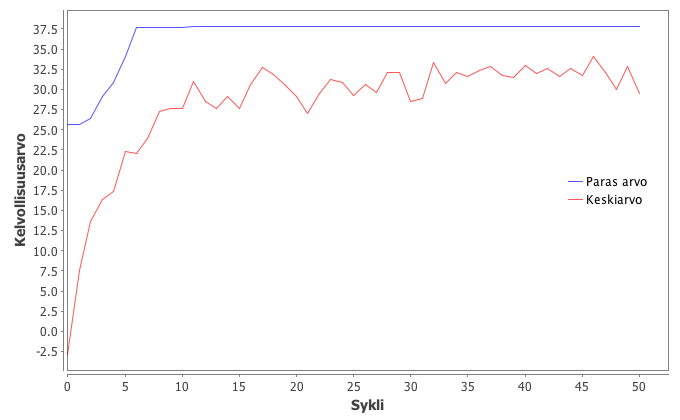
\includegraphics[width=12cm]{1_ranked_tournament}
	\label{fig:1_ranked_tournament}
\end{figure}
